% **************************************************************************************************************
% A Classic Thesis Style
% An Homage to The Elements of Typographic Style
%
% Copyright (C) 2015 André Miede http://www.miede.de
%
% If you like the style then I would appreciate a postcard. My address
% can be found in the file ClassicThesis.pdf. A collection of the
% postcards I received so far is available online at
% http://postcards.miede.de
%
% License:
% This program is free software; you can redistribute it and/or modify
% it under the terms of the GNU General Public License as published by
% the Free Software Foundation; either version 2 of the License, or
% (at your option) any later version.
%
% This program is distributed in the hope that it will be useful,
% but WITHOUT ANY WARRANTY; without even the implied warranty of
% MERCHANTABILITY or FITNESS FOR A PARTICULAR PURPOSE.  See the
% GNU General Public License for more details.
%
% You should have received a copy of the GNU General Public License
% along with this program; see the file COPYING.  If not, write to
% the Free Software Foundation, Inc., 59 Temple Place - Suite 330,
% Boston, MA 02111-1307, USA.
%
% **************************************************************************************************************
\RequirePackage{fix-cm} % fix some latex issues see: http://texdoc.net/texmf-dist/doc/latex/base/fixltx2e.pdf
\documentclass[ twoside,openright,titlepage,numbers=noenddot,headinclude,%1headlines,% letterpaper a4paper
                footinclude=true,cleardoublepage=empty,abstractoff, % <--- obsolete, remove (todo)
                BCOR=5mm,paper=a4,fontsize=11pt,a4paper,%
                british,ngerman,%
                ]{scrreprt}

%********************************************************************
% Note: Make all your adjustments in here
%*******************************************************
%Added by Stefan Huber
\usepackage{comment}
\usepackage[dvipsnames]{xcolor}
\usepackage{minted} % should be added before scrhack %newfloat now working
\usepackage{wrapfig}
\usepackage{smartdiagram}
\usesmartdiagramlibrary{additions}

% ****************************************************************************************************
% classicthesis-config.tex
% formerly known as loadpackages.sty, classicthesis-ldpkg.sty, and classicthesis-preamble.sty
% Use it at the beginning of your ClassicThesis.tex, or as a LaTeX Preamble
% in your ClassicThesis.{tex,lyx} with %Added by Stefan Huber
\usepackage{comment}
\usepackage[dvipsnames]{xcolor}
\usepackage{minted} % should be added before scrhack %newfloat now working
\usepackage{wrapfig}
\usepackage{smartdiagram}
\usesmartdiagramlibrary{additions}

% ****************************************************************************************************
% classicthesis-config.tex
% formerly known as loadpackages.sty, classicthesis-ldpkg.sty, and classicthesis-preamble.sty
% Use it at the beginning of your ClassicThesis.tex, or as a LaTeX Preamble
% in your ClassicThesis.{tex,lyx} with %Added by Stefan Huber
\usepackage{comment}
\usepackage[dvipsnames]{xcolor}
\usepackage{minted} % should be added before scrhack %newfloat now working
\usepackage{wrapfig}
\usepackage{smartdiagram}
\usesmartdiagramlibrary{additions}

% ****************************************************************************************************
% classicthesis-config.tex
% formerly known as loadpackages.sty, classicthesis-ldpkg.sty, and classicthesis-preamble.sty
% Use it at the beginning of your ClassicThesis.tex, or as a LaTeX Preamble
% in your ClassicThesis.{tex,lyx} with \input{classicthesis-config}
% ****************************************************************************************************
% If you like the classicthesis, then I would appreciate a postcard.
% My address can be found in the file ClassicThesis.pdf. A collection
% of the postcards I received so far is available online at
% http://postcards.miede.de
% ****************************************************************************************************


% ****************************************************************************************************
% 0. Set the encoding of your files. UTF-8 is the only sensible encoding nowadays. If you can't read
% äöüßáéçèê∂åëæƒÏ€ then change the encoding setting in your editor, not the line below. If your editor
% does not support utf8 use another editor!
% ****************************************************************************************************
\PassOptionsToPackage{utf8}{inputenc}
\usepackage{inputenc}

% ****************************************************************************************************
% 1. Configure classicthesis for your needs here, e.g., remove "drafting" below
% in order to deactivate the time-stamp on the pages
% ****************************************************************************************************
\PassOptionsToPackage{eulerchapternumbers,listings,%drafting,%
        pdfspacing,%floatperchapter,%linedheaders,%
        dottedtoc,
        subfig,beramono,eulermath,parts}{classicthesis}
% ********************************************************************
% Available options for classicthesis.sty
% (see ClassicThesis.pdf for more information):
% drafting
% parts nochapters linedheaders
% eulerchapternumbers beramono eulermath pdfspacing minionprospacing
% tocaligned dottedtoc manychapters
% listings floatperchapter subfig
% ********************************************************************


% ****************************************************************************************************
% 2. Personal data and user ad-hoc commands
% ****************************************************************************************************
\newcommand{\myTitle}{A Classic Thesis Style\xspace}
\newcommand{\mySubtitle}{An Homage to The Elements of Typographic Style\xspace}
\newcommand{\myDegree}{Nahe am Bachelor\xspace}
\newcommand{\myName}{Stefan Huber\xspace}
\newcommand{\myProf}{Put name here\xspace}
\newcommand{\myOtherProf}{Put name here\xspace}
\newcommand{\mySupervisor}{Andreas Simbürger\xspace}
\newcommand{\myFaculty}{Fakultät für Informatik und Mathematik\xspace}
\newcommand{\myDepartment}{Department\xspace}
\newcommand{\myUni}{Universität Passau\xspace}
\newcommand{\myLocation}{Passau\xspace}
\newcommand{\myTime}{September 2017\xspace}
\newcommand{\myVersion}{version 1\xspace}

% ********************************************************************
% Setup, finetuning, and useful commands
% ********************************************************************
\newcounter{dummy} % necessary for correct hyperlinks (to index, bib, etc.)
\newlength{\abcd} % for ab..z string length calculation
\providecommand{\mLyX}{L\kern-.1667em\lower.25em\hbox{Y}\kern-.125emX\@}
\newcommand{\eg}{e.\,g.}
\newcommand{\Eg}{E.\,g.}
% ****************************************************************************************************


% ****************************************************************************************************
% 3. Loading some handy packages
% ****************************************************************************************************
% ********************************************************************
% Packages with options that might require adjustments
% ********************************************************************
\PassOptionsToPackage{british}{babel}   % change this to your language(s)
% Spanish languages need extra options in order to work with this template
%\PassOptionsToPackage{spanish,es-lcroman}{babel}
\usepackage{babel}

\usepackage{csquotes}
\PassOptionsToPackage{%
    %backend=biber, %instead of bibtex
    backend=bibtex8,bibencoding=ascii,%
    language=auto,%
    style=numeric-comp,%
    %style=authoryear-comp, % Author 1999, 2010
    %bibstyle=authoryear,dashed=false, % dashed: substitute rep. author with ---
    sorting=nyt, % name, year, title
    maxbibnames=10, % default: 3, et al.
    %backref=true,%
    natbib=true % natbib compatibility mode (\citep and \citet still work)
}{biblatex}
    \usepackage{biblatex}

\PassOptionsToPackage{fleqn}{amsmath}       % math environments and more by the AMS
    \usepackage{amsmath}

% ********************************************************************
% General useful packages
% ********************************************************************
\PassOptionsToPackage{T1}{fontenc} % T2A for cyrillics
    \usepackage{fontenc}
\usepackage{textcomp} % fix warning with missing font shapes
\usepackage{scrhack} % fix warnings when using KOMA with listings package
\usepackage{xspace} % to get the spacing after macros right
\usepackage{mparhack} % get marginpar right
\usepackage{fixltx2e} % fixes some LaTeX stuff --> since 2015 in the LaTeX kernel (see below)
%\usepackage[latest]{latexrelease} % will be used once available in more distributions (ISSUE #107)
\PassOptionsToPackage{printonlyused,smaller}{acronym}
    \usepackage{acronym} % nice macros for handling all acronyms in the thesis
    %\renewcommand{\bflabel}[1]{{#1}\hfill} % fix the list of acronyms --> no longer working
    %\renewcommand*{\acsfont}[1]{\textsc{#1}}
    \renewcommand*{\aclabelfont}[1]{\acsfont{#1}}
% ****************************************************************************************************


% ****************************************************************************************************
% 4. Setup floats: tables, (sub)figures, and captions
% ****************************************************************************************************
\usepackage{tabularx} % better tables
    \setlength{\extrarowheight}{3pt} % increase table row height
\newcommand{\tableheadline}[1]{\multicolumn{1}{c}{\spacedlowsmallcaps{#1}}}
\newcommand{\myfloatalign}{\centering} % to be used with each float for alignment
\usepackage{caption}
% Thanks to cgnieder and Claus Lahiri
% http://tex.stackexchange.com/questions/69349/spacedlowsmallcaps-in-caption-label
% [REMOVED DUE TO OTHER PROBLEMS, SEE ISSUE #82]
%\DeclareCaptionLabelFormat{smallcaps}{\bothIfFirst{#1}{~}\MakeTextLowercase{\textsc{#2}}}
%\captionsetup{font=small,labelformat=smallcaps} % format=hang,
\captionsetup{font=small} % format=hang,
\usepackage{subfig}
% ****************************************************************************************************


% ****************************************************************************************************
% 5. Setup code listings
% ****************************************************************************************************
\begin{comment}
    \usepackage{listings}
    %\lstset{emph={trueIndex,root},emphstyle=\color{BlueViolet}}%\underbar} % for special keywords
    \lstset{language=C++,
        morekeywords={PassOptionsToPackage,selectlanguage},
        keywordstyle=\color{NavyBlue},%\bfseries,
        basicstyle=\small\ttfamily,
        %identifierstyle=\color{NavyBlue},
        commentstyle=\color{Green}\ttfamily,
        stringstyle=\rmfamily,
        numbers=left,
        numberstyle=\scriptsize,%\tiny
        %stepnumber=5,
        numbersep=8pt,
        showstringspaces=false,
        breaklines=true,
        %frameround=ftff,
        %frame=single,
        belowcaptionskip=.75\baselineskip,
        frame=L
    }
\end{comment}
% ****************************************************************************************************


% ****************************************************************************************************
% 6. PDFLaTeX, hyperreferences and citation backreferences
% ****************************************************************************************************
% ********************************************************************
% Using PDFLaTeX
% ********************************************************************
\PassOptionsToPackage{pdftex,hyperfootnotes=false,pdfpagelabels}{hyperref}
    \usepackage{hyperref}  % backref linktocpage pagebackref
\pdfcompresslevel=9
\pdfadjustspacing=1
\PassOptionsToPackage{pdftex}{graphicx}
    \usepackage{graphicx}


% ********************************************************************
% Hyperreferences
% ********************************************************************
\hypersetup{%
    %draft, % = no hyperlinking at all (useful in b/w printouts)
    colorlinks=true, linktocpage=true, pdfstartpage=3, pdfstartview=FitV,%
    % uncomment the following line if you want to have black links (e.g., for printing)
    %colorlinks=false, linktocpage=false, pdfstartpage=3, pdfstartview=FitV, pdfborder={0 0 0},%
    breaklinks=true, pdfpagemode=UseNone, pageanchor=true, pdfpagemode=UseOutlines,%
    plainpages=false, bookmarksnumbered, bookmarksopen=true, bookmarksopenlevel=1,%
    hypertexnames=true, pdfhighlight=/O,%nesting=true,%frenchlinks,%
    urlcolor=webbrown, linkcolor=RoyalBlue, citecolor=webgreen, %pagecolor=RoyalBlue,%
    %urlcolor=Black, linkcolor=Black, citecolor=Black, %pagecolor=Black,%
    pdftitle={\myTitle},%
    pdfauthor={\textcopyright\ \myName, \myUni, \myFaculty},%
    pdfsubject={},%
    pdfkeywords={},%
    pdfcreator={pdfLaTeX},%
    pdfproducer={LaTeX with hyperref and classicthesis}%
}

% ********************************************************************
% Setup autoreferences
% ********************************************************************
% There are some issues regarding autorefnames
% http://www.ureader.de/msg/136221647.aspx
% http://www.tex.ac.uk/cgi-bin/texfaq2html?label=latexwords
% you have to redefine the makros for the
% language you use, e.g., american, ngerman
% (as chosen when loading babel/AtBeginDocument)
% ********************************************************************
\makeatletter
\@ifpackageloaded{babel}%
    {%
        \addto\extrasamerican{%
            \renewcommand*{\figureautorefname}{Figure}%
            \renewcommand*{\tableautorefname}{Table}%
            \renewcommand*{\partautorefname}{Part}%
            \renewcommand*{\chapterautorefname}{Chapter}%
            \renewcommand*{\sectionautorefname}{Section}%
            \renewcommand*{\subsectionautorefname}{Section}%
            \renewcommand*{\subsubsectionautorefname}{Section}%
        }%
        \addto\extrasbritish{%
            \renewcommand*{\figureautorefname}{Figure}%
            \renewcommand*{\tableautorefname}{Table}%
            \renewcommand*{\partautorefname}{Part}%
            \renewcommand*{\chapterautorefname}{Chapter}%
            \renewcommand*{\sectionautorefname}{Section}%
            \renewcommand*{\subsectionautorefname}{Section}%
            \renewcommand*{\subsubsectionautorefname}{Section}%
        }%
        \addto\extrasngerman{%
            \renewcommand*{\paragraphautorefname}{Absatz}%
            \renewcommand*{\subparagraphautorefname}{Unterabsatz}%
            \renewcommand*{\footnoteautorefname}{Fu\"snote}%
            \renewcommand*{\FancyVerbLineautorefname}{Zeile}%
            \renewcommand*{\theoremautorefname}{Theorem}%
            \renewcommand*{\appendixautorefname}{Anhang}%
            \renewcommand*{\equationautorefname}{Gleichung}%
            \renewcommand*{\itemautorefname}{Punkt}%
        }%
        % Fix to getting autorefs for subfigures right (thanks to Belinda Vogt for changing the definition)
        \providecommand{\subfigureautorefname}{\figureautorefname}%
    }{\relax}
\makeatother


% ****************************************************************************************************
% 7. Last calls before the bar closes
% ****************************************************************************************************
% ********************************************************************
% Development Stuff
% ********************************************************************
\listfiles
%\PassOptionsToPackage{l2tabu,orthodox,abort}{nag}
%   \usepackage{nag}
%\PassOptionsToPackage{warning, all}{onlyamsmath}
%   \usepackage{onlyamsmath}

% ********************************************************************
% Last, but not least...
% ********************************************************************
\usepackage{classicthesis}
% ****************************************************************************************************


% ****************************************************************************************************
% 8. Further adjustments (experimental)
% ****************************************************************************************************
% ********************************************************************
% Changing the text area
% ********************************************************************
%\linespread{1.05} % a bit more for Palatino
%\areaset[current]{312pt}{761pt} % 686 (factor 2.2) + 33 head + 42 head \the\footskip
%\setlength{\marginparwidth}{7em}%
%\setlength{\marginparsep}{2em}%

% ********************************************************************
% Using different fonts
% ********************************************************************
%\usepackage[oldstylenums]{kpfonts} % oldstyle notextcomp
%\usepackage[osf]{libertine}
%\usepackage[light,condensed,math]{iwona}
%\renewcommand{\sfdefault}{iwona}
%\usepackage{lmodern} % <-- no osf support :-(
%\usepackage{cfr-lm} %
%\usepackage[urw-garamond]{mathdesign} <-- no osf support :-(
%\usepackage[default,osfigures]{opensans} % scale=0.95
%\usepackage[sfdefault]{FiraSans}
% ****************************************************************************************************


%Customization Stefan Huber
%custom colors
\definecolor{defaultColor}{HTML}{1E90FF}
\definecolor{llvmIrColor}{HTML}{228B22}
\definecolor{nonLlvmIrColor}{HTML}{B22222}

%minted configure
\setminted{
    linenos,
    breaklines
}
\providecommand*{\listingautorefname}{Listing}
\newenvironment{code}{\captionsetup{type=listing}}{}
%\SetupFloatingEnvironment{listing}{name=Program code} %newfloat package
%\renewcommand{\listoflistingscaption}{List of Program Code} %float package

%Tikz
\usepackage{tikz}
\usetikzlibrary{arrows.meta, positioning, shapes, snakes, fit}
\tikzset{
    node distance = 5mm and 15mm,
    defaultNode/.style = {rectangle, rounded corners, draw=gray, drop shadow, very thick, bottom color=defaultColor!50!white, text centered, top color=white, minimum height=1.2em, minimum width=3em},
    llvmIrNode/.style = {defaultNode, bottom color=llvmIrColor!50!white},
    nonLlvmIrNode/.style = {defaultNode, bottom color=nonLlvmIrColor!50!white},
    legendNode/.style = {rectangle},
    defaultPath/.style = {-{Stealth[length=4mm]}, color=defaultColor, line width=0.2em, draw, rounded corners},
    llvmIrPath/.style = {defaultPath, color=llvmIrColor},
    nonLlvmIrPath/.style = {defaultPath, color=nonLlvmIrColor}
}
\newcommand{\legend}[0]{
    \begin{tikzpicture}
        \coordinate (firstRowCenter);
        \coordinate[left=of firstRowCenter] (firstRowLeft);
        \coordinate[right=of firstRowCenter] (firstRowRight);
        \path[llvmIrPath] (firstRowLeft) to (firstRowRight);
        \node[legendNode, right=of firstRowRight] {Passing LLVM-IR};

        \node[llvmIrNode, below=of firstRowCenter] (secondRowCenter) {Node};
        \coordinate[left=of secondRowCenter] (secondRowLeft);
        \coordinate[right=of secondRowCenter] (secondRowRight);
        \node[legendNode, right=of secondRowRight] {Node using LLVM-IR};

        \coordinate[below=of secondRowCenter] (thirdRowCenter);
        \coordinate[left=of thirdRowCenter] (thirdRowLeft);
        \coordinate[right=of thirdRowCenter] (thirdRowRight);
        \path[nonLlvmIrPath] (thirdRowLeft) to (thirdRowRight);
        \node[legendNode, right=of thirdRowRight] {Passing non-LLVM-IR};

        \node[nonLlvmIrNode, below=of thirdRowCenter] (fourthRowCenter) {Node};
        \coordinate[left=of fourthRowCenter] (fourthRowLeft);
        \coordinate[right=of fourthRowCenter] (fourthRowRight);
        \node[legendNode, right=of fourthRowRight] {Node not using LLVM-IR};
    \end{tikzpicture}
}

%Shortcuts
\newcommand{\cfg}{\ac{CFG} }
\newcommand{\scop}{\ac{SCoP} }
\newcommand{\scops}{\ac{SCoP}s }
\newcommand{\llvmir}{\ac{LLVM-IR} }
\newcommand{\llvm}{\ac{LLVM} }
\newcommand{\opt}{LLVM Optimizer }
\newcommand{\generator}{LLVM Code Generator }
\newcommand{\linker}{LLVM Linker }

%temporary commands while drafting
\newcommand{\draftnote}[1]{\textit{\textbf{\textcolor{red}{#1}}}}

% ****************************************************************************************************
% If you like the classicthesis, then I would appreciate a postcard.
% My address can be found in the file ClassicThesis.pdf. A collection
% of the postcards I received so far is available online at
% http://postcards.miede.de
% ****************************************************************************************************


% ****************************************************************************************************
% 0. Set the encoding of your files. UTF-8 is the only sensible encoding nowadays. If you can't read
% äöüßáéçèê∂åëæƒÏ€ then change the encoding setting in your editor, not the line below. If your editor
% does not support utf8 use another editor!
% ****************************************************************************************************
\PassOptionsToPackage{utf8}{inputenc}
\usepackage{inputenc}

% ****************************************************************************************************
% 1. Configure classicthesis for your needs here, e.g., remove "drafting" below
% in order to deactivate the time-stamp on the pages
% ****************************************************************************************************
\PassOptionsToPackage{eulerchapternumbers,listings,%drafting,%
        pdfspacing,%floatperchapter,%linedheaders,%
        dottedtoc,
        subfig,beramono,eulermath,parts}{classicthesis}
% ********************************************************************
% Available options for classicthesis.sty
% (see ClassicThesis.pdf for more information):
% drafting
% parts nochapters linedheaders
% eulerchapternumbers beramono eulermath pdfspacing minionprospacing
% tocaligned dottedtoc manychapters
% listings floatperchapter subfig
% ********************************************************************


% ****************************************************************************************************
% 2. Personal data and user ad-hoc commands
% ****************************************************************************************************
\newcommand{\myTitle}{A Classic Thesis Style\xspace}
\newcommand{\mySubtitle}{An Homage to The Elements of Typographic Style\xspace}
\newcommand{\myDegree}{Nahe am Bachelor\xspace}
\newcommand{\myName}{Stefan Huber\xspace}
\newcommand{\myProf}{Put name here\xspace}
\newcommand{\myOtherProf}{Put name here\xspace}
\newcommand{\mySupervisor}{Andreas Simbürger\xspace}
\newcommand{\myFaculty}{Fakultät für Informatik und Mathematik\xspace}
\newcommand{\myDepartment}{Department\xspace}
\newcommand{\myUni}{Universität Passau\xspace}
\newcommand{\myLocation}{Passau\xspace}
\newcommand{\myTime}{September 2017\xspace}
\newcommand{\myVersion}{version 1\xspace}

% ********************************************************************
% Setup, finetuning, and useful commands
% ********************************************************************
\newcounter{dummy} % necessary for correct hyperlinks (to index, bib, etc.)
\newlength{\abcd} % for ab..z string length calculation
\providecommand{\mLyX}{L\kern-.1667em\lower.25em\hbox{Y}\kern-.125emX\@}
\newcommand{\eg}{e.\,g.}
\newcommand{\Eg}{E.\,g.}
% ****************************************************************************************************


% ****************************************************************************************************
% 3. Loading some handy packages
% ****************************************************************************************************
% ********************************************************************
% Packages with options that might require adjustments
% ********************************************************************
\PassOptionsToPackage{british}{babel}   % change this to your language(s)
% Spanish languages need extra options in order to work with this template
%\PassOptionsToPackage{spanish,es-lcroman}{babel}
\usepackage{babel}

\usepackage{csquotes}
\PassOptionsToPackage{%
    %backend=biber, %instead of bibtex
    backend=bibtex8,bibencoding=ascii,%
    language=auto,%
    style=numeric-comp,%
    %style=authoryear-comp, % Author 1999, 2010
    %bibstyle=authoryear,dashed=false, % dashed: substitute rep. author with ---
    sorting=nyt, % name, year, title
    maxbibnames=10, % default: 3, et al.
    %backref=true,%
    natbib=true % natbib compatibility mode (\citep and \citet still work)
}{biblatex}
    \usepackage{biblatex}

\PassOptionsToPackage{fleqn}{amsmath}       % math environments and more by the AMS
    \usepackage{amsmath}

% ********************************************************************
% General useful packages
% ********************************************************************
\PassOptionsToPackage{T1}{fontenc} % T2A for cyrillics
    \usepackage{fontenc}
\usepackage{textcomp} % fix warning with missing font shapes
\usepackage{scrhack} % fix warnings when using KOMA with listings package
\usepackage{xspace} % to get the spacing after macros right
\usepackage{mparhack} % get marginpar right
\usepackage{fixltx2e} % fixes some LaTeX stuff --> since 2015 in the LaTeX kernel (see below)
%\usepackage[latest]{latexrelease} % will be used once available in more distributions (ISSUE #107)
\PassOptionsToPackage{printonlyused,smaller}{acronym}
    \usepackage{acronym} % nice macros for handling all acronyms in the thesis
    %\renewcommand{\bflabel}[1]{{#1}\hfill} % fix the list of acronyms --> no longer working
    %\renewcommand*{\acsfont}[1]{\textsc{#1}}
    \renewcommand*{\aclabelfont}[1]{\acsfont{#1}}
% ****************************************************************************************************


% ****************************************************************************************************
% 4. Setup floats: tables, (sub)figures, and captions
% ****************************************************************************************************
\usepackage{tabularx} % better tables
    \setlength{\extrarowheight}{3pt} % increase table row height
\newcommand{\tableheadline}[1]{\multicolumn{1}{c}{\spacedlowsmallcaps{#1}}}
\newcommand{\myfloatalign}{\centering} % to be used with each float for alignment
\usepackage{caption}
% Thanks to cgnieder and Claus Lahiri
% http://tex.stackexchange.com/questions/69349/spacedlowsmallcaps-in-caption-label
% [REMOVED DUE TO OTHER PROBLEMS, SEE ISSUE #82]
%\DeclareCaptionLabelFormat{smallcaps}{\bothIfFirst{#1}{~}\MakeTextLowercase{\textsc{#2}}}
%\captionsetup{font=small,labelformat=smallcaps} % format=hang,
\captionsetup{font=small} % format=hang,
\usepackage{subfig}
% ****************************************************************************************************


% ****************************************************************************************************
% 5. Setup code listings
% ****************************************************************************************************
\begin{comment}
    \usepackage{listings}
    %\lstset{emph={trueIndex,root},emphstyle=\color{BlueViolet}}%\underbar} % for special keywords
    \lstset{language=C++,
        morekeywords={PassOptionsToPackage,selectlanguage},
        keywordstyle=\color{NavyBlue},%\bfseries,
        basicstyle=\small\ttfamily,
        %identifierstyle=\color{NavyBlue},
        commentstyle=\color{Green}\ttfamily,
        stringstyle=\rmfamily,
        numbers=left,
        numberstyle=\scriptsize,%\tiny
        %stepnumber=5,
        numbersep=8pt,
        showstringspaces=false,
        breaklines=true,
        %frameround=ftff,
        %frame=single,
        belowcaptionskip=.75\baselineskip,
        frame=L
    }
\end{comment}
% ****************************************************************************************************


% ****************************************************************************************************
% 6. PDFLaTeX, hyperreferences and citation backreferences
% ****************************************************************************************************
% ********************************************************************
% Using PDFLaTeX
% ********************************************************************
\PassOptionsToPackage{pdftex,hyperfootnotes=false,pdfpagelabels}{hyperref}
    \usepackage{hyperref}  % backref linktocpage pagebackref
\pdfcompresslevel=9
\pdfadjustspacing=1
\PassOptionsToPackage{pdftex}{graphicx}
    \usepackage{graphicx}


% ********************************************************************
% Hyperreferences
% ********************************************************************
\hypersetup{%
    %draft, % = no hyperlinking at all (useful in b/w printouts)
    colorlinks=true, linktocpage=true, pdfstartpage=3, pdfstartview=FitV,%
    % uncomment the following line if you want to have black links (e.g., for printing)
    %colorlinks=false, linktocpage=false, pdfstartpage=3, pdfstartview=FitV, pdfborder={0 0 0},%
    breaklinks=true, pdfpagemode=UseNone, pageanchor=true, pdfpagemode=UseOutlines,%
    plainpages=false, bookmarksnumbered, bookmarksopen=true, bookmarksopenlevel=1,%
    hypertexnames=true, pdfhighlight=/O,%nesting=true,%frenchlinks,%
    urlcolor=webbrown, linkcolor=RoyalBlue, citecolor=webgreen, %pagecolor=RoyalBlue,%
    %urlcolor=Black, linkcolor=Black, citecolor=Black, %pagecolor=Black,%
    pdftitle={\myTitle},%
    pdfauthor={\textcopyright\ \myName, \myUni, \myFaculty},%
    pdfsubject={},%
    pdfkeywords={},%
    pdfcreator={pdfLaTeX},%
    pdfproducer={LaTeX with hyperref and classicthesis}%
}

% ********************************************************************
% Setup autoreferences
% ********************************************************************
% There are some issues regarding autorefnames
% http://www.ureader.de/msg/136221647.aspx
% http://www.tex.ac.uk/cgi-bin/texfaq2html?label=latexwords
% you have to redefine the makros for the
% language you use, e.g., american, ngerman
% (as chosen when loading babel/AtBeginDocument)
% ********************************************************************
\makeatletter
\@ifpackageloaded{babel}%
    {%
        \addto\extrasamerican{%
            \renewcommand*{\figureautorefname}{Figure}%
            \renewcommand*{\tableautorefname}{Table}%
            \renewcommand*{\partautorefname}{Part}%
            \renewcommand*{\chapterautorefname}{Chapter}%
            \renewcommand*{\sectionautorefname}{Section}%
            \renewcommand*{\subsectionautorefname}{Section}%
            \renewcommand*{\subsubsectionautorefname}{Section}%
        }%
        \addto\extrasbritish{%
            \renewcommand*{\figureautorefname}{Figure}%
            \renewcommand*{\tableautorefname}{Table}%
            \renewcommand*{\partautorefname}{Part}%
            \renewcommand*{\chapterautorefname}{Chapter}%
            \renewcommand*{\sectionautorefname}{Section}%
            \renewcommand*{\subsectionautorefname}{Section}%
            \renewcommand*{\subsubsectionautorefname}{Section}%
        }%
        \addto\extrasngerman{%
            \renewcommand*{\paragraphautorefname}{Absatz}%
            \renewcommand*{\subparagraphautorefname}{Unterabsatz}%
            \renewcommand*{\footnoteautorefname}{Fu\"snote}%
            \renewcommand*{\FancyVerbLineautorefname}{Zeile}%
            \renewcommand*{\theoremautorefname}{Theorem}%
            \renewcommand*{\appendixautorefname}{Anhang}%
            \renewcommand*{\equationautorefname}{Gleichung}%
            \renewcommand*{\itemautorefname}{Punkt}%
        }%
        % Fix to getting autorefs for subfigures right (thanks to Belinda Vogt for changing the definition)
        \providecommand{\subfigureautorefname}{\figureautorefname}%
    }{\relax}
\makeatother


% ****************************************************************************************************
% 7. Last calls before the bar closes
% ****************************************************************************************************
% ********************************************************************
% Development Stuff
% ********************************************************************
\listfiles
%\PassOptionsToPackage{l2tabu,orthodox,abort}{nag}
%   \usepackage{nag}
%\PassOptionsToPackage{warning, all}{onlyamsmath}
%   \usepackage{onlyamsmath}

% ********************************************************************
% Last, but not least...
% ********************************************************************
\usepackage{classicthesis}
% ****************************************************************************************************


% ****************************************************************************************************
% 8. Further adjustments (experimental)
% ****************************************************************************************************
% ********************************************************************
% Changing the text area
% ********************************************************************
%\linespread{1.05} % a bit more for Palatino
%\areaset[current]{312pt}{761pt} % 686 (factor 2.2) + 33 head + 42 head \the\footskip
%\setlength{\marginparwidth}{7em}%
%\setlength{\marginparsep}{2em}%

% ********************************************************************
% Using different fonts
% ********************************************************************
%\usepackage[oldstylenums]{kpfonts} % oldstyle notextcomp
%\usepackage[osf]{libertine}
%\usepackage[light,condensed,math]{iwona}
%\renewcommand{\sfdefault}{iwona}
%\usepackage{lmodern} % <-- no osf support :-(
%\usepackage{cfr-lm} %
%\usepackage[urw-garamond]{mathdesign} <-- no osf support :-(
%\usepackage[default,osfigures]{opensans} % scale=0.95
%\usepackage[sfdefault]{FiraSans}
% ****************************************************************************************************


%Customization Stefan Huber
%custom colors
\definecolor{defaultColor}{HTML}{1E90FF}
\definecolor{llvmIrColor}{HTML}{228B22}
\definecolor{nonLlvmIrColor}{HTML}{B22222}

%minted configure
\setminted{
    linenos,
    breaklines
}
\providecommand*{\listingautorefname}{Listing}
\newenvironment{code}{\captionsetup{type=listing}}{}
%\SetupFloatingEnvironment{listing}{name=Program code} %newfloat package
%\renewcommand{\listoflistingscaption}{List of Program Code} %float package

%Tikz
\usepackage{tikz}
\usetikzlibrary{arrows.meta, positioning, shapes, snakes, fit}
\tikzset{
    node distance = 5mm and 15mm,
    defaultNode/.style = {rectangle, rounded corners, draw=gray, drop shadow, very thick, bottom color=defaultColor!50!white, text centered, top color=white, minimum height=1.2em, minimum width=3em},
    llvmIrNode/.style = {defaultNode, bottom color=llvmIrColor!50!white},
    nonLlvmIrNode/.style = {defaultNode, bottom color=nonLlvmIrColor!50!white},
    legendNode/.style = {rectangle},
    defaultPath/.style = {-{Stealth[length=4mm]}, color=defaultColor, line width=0.2em, draw, rounded corners},
    llvmIrPath/.style = {defaultPath, color=llvmIrColor},
    nonLlvmIrPath/.style = {defaultPath, color=nonLlvmIrColor}
}
\newcommand{\legend}[0]{
    \begin{tikzpicture}
        \coordinate (firstRowCenter);
        \coordinate[left=of firstRowCenter] (firstRowLeft);
        \coordinate[right=of firstRowCenter] (firstRowRight);
        \path[llvmIrPath] (firstRowLeft) to (firstRowRight);
        \node[legendNode, right=of firstRowRight] {Passing LLVM-IR};

        \node[llvmIrNode, below=of firstRowCenter] (secondRowCenter) {Node};
        \coordinate[left=of secondRowCenter] (secondRowLeft);
        \coordinate[right=of secondRowCenter] (secondRowRight);
        \node[legendNode, right=of secondRowRight] {Node using LLVM-IR};

        \coordinate[below=of secondRowCenter] (thirdRowCenter);
        \coordinate[left=of thirdRowCenter] (thirdRowLeft);
        \coordinate[right=of thirdRowCenter] (thirdRowRight);
        \path[nonLlvmIrPath] (thirdRowLeft) to (thirdRowRight);
        \node[legendNode, right=of thirdRowRight] {Passing non-LLVM-IR};

        \node[nonLlvmIrNode, below=of thirdRowCenter] (fourthRowCenter) {Node};
        \coordinate[left=of fourthRowCenter] (fourthRowLeft);
        \coordinate[right=of fourthRowCenter] (fourthRowRight);
        \node[legendNode, right=of fourthRowRight] {Node not using LLVM-IR};
    \end{tikzpicture}
}

%Shortcuts
\newcommand{\cfg}{\ac{CFG} }
\newcommand{\scop}{\ac{SCoP} }
\newcommand{\scops}{\ac{SCoP}s }
\newcommand{\llvmir}{\ac{LLVM-IR} }
\newcommand{\llvm}{\ac{LLVM} }
\newcommand{\opt}{LLVM Optimizer }
\newcommand{\generator}{LLVM Code Generator }
\newcommand{\linker}{LLVM Linker }

%temporary commands while drafting
\newcommand{\draftnote}[1]{\textit{\textbf{\textcolor{red}{#1}}}}

% ****************************************************************************************************
% If you like the classicthesis, then I would appreciate a postcard.
% My address can be found in the file ClassicThesis.pdf. A collection
% of the postcards I received so far is available online at
% http://postcards.miede.de
% ****************************************************************************************************


% ****************************************************************************************************
% 0. Set the encoding of your files. UTF-8 is the only sensible encoding nowadays. If you can't read
% äöüßáéçèê∂åëæƒÏ€ then change the encoding setting in your editor, not the line below. If your editor
% does not support utf8 use another editor!
% ****************************************************************************************************
\PassOptionsToPackage{utf8}{inputenc}
\usepackage{inputenc}

% ****************************************************************************************************
% 1. Configure classicthesis for your needs here, e.g., remove "drafting" below
% in order to deactivate the time-stamp on the pages
% ****************************************************************************************************
\PassOptionsToPackage{eulerchapternumbers,listings,%drafting,%
        pdfspacing,%floatperchapter,%linedheaders,%
        dottedtoc,
        subfig,beramono,eulermath,parts}{classicthesis}
% ********************************************************************
% Available options for classicthesis.sty
% (see ClassicThesis.pdf for more information):
% drafting
% parts nochapters linedheaders
% eulerchapternumbers beramono eulermath pdfspacing minionprospacing
% tocaligned dottedtoc manychapters
% listings floatperchapter subfig
% ********************************************************************


% ****************************************************************************************************
% 2. Personal data and user ad-hoc commands
% ****************************************************************************************************
\newcommand{\myTitle}{A Classic Thesis Style\xspace}
\newcommand{\mySubtitle}{An Homage to The Elements of Typographic Style\xspace}
\newcommand{\myDegree}{Nahe am Bachelor\xspace}
\newcommand{\myName}{Stefan Huber\xspace}
\newcommand{\myProf}{Put name here\xspace}
\newcommand{\myOtherProf}{Put name here\xspace}
\newcommand{\mySupervisor}{Andreas Simbürger\xspace}
\newcommand{\myFaculty}{Fakultät für Informatik und Mathematik\xspace}
\newcommand{\myDepartment}{Department\xspace}
\newcommand{\myUni}{Universität Passau\xspace}
\newcommand{\myLocation}{Passau\xspace}
\newcommand{\myTime}{September 2017\xspace}
\newcommand{\myVersion}{version 1\xspace}

% ********************************************************************
% Setup, finetuning, and useful commands
% ********************************************************************
\newcounter{dummy} % necessary for correct hyperlinks (to index, bib, etc.)
\newlength{\abcd} % for ab..z string length calculation
\providecommand{\mLyX}{L\kern-.1667em\lower.25em\hbox{Y}\kern-.125emX\@}
\newcommand{\eg}{e.\,g.}
\newcommand{\Eg}{E.\,g.}
% ****************************************************************************************************


% ****************************************************************************************************
% 3. Loading some handy packages
% ****************************************************************************************************
% ********************************************************************
% Packages with options that might require adjustments
% ********************************************************************
\PassOptionsToPackage{british}{babel}   % change this to your language(s)
% Spanish languages need extra options in order to work with this template
%\PassOptionsToPackage{spanish,es-lcroman}{babel}
\usepackage{babel}

\usepackage{csquotes}
\PassOptionsToPackage{%
    %backend=biber, %instead of bibtex
    backend=bibtex8,bibencoding=ascii,%
    language=auto,%
    style=numeric-comp,%
    %style=authoryear-comp, % Author 1999, 2010
    %bibstyle=authoryear,dashed=false, % dashed: substitute rep. author with ---
    sorting=nyt, % name, year, title
    maxbibnames=10, % default: 3, et al.
    %backref=true,%
    natbib=true % natbib compatibility mode (\citep and \citet still work)
}{biblatex}
    \usepackage{biblatex}

\PassOptionsToPackage{fleqn}{amsmath}       % math environments and more by the AMS
    \usepackage{amsmath}

% ********************************************************************
% General useful packages
% ********************************************************************
\PassOptionsToPackage{T1}{fontenc} % T2A for cyrillics
    \usepackage{fontenc}
\usepackage{textcomp} % fix warning with missing font shapes
\usepackage{scrhack} % fix warnings when using KOMA with listings package
\usepackage{xspace} % to get the spacing after macros right
\usepackage{mparhack} % get marginpar right
\usepackage{fixltx2e} % fixes some LaTeX stuff --> since 2015 in the LaTeX kernel (see below)
%\usepackage[latest]{latexrelease} % will be used once available in more distributions (ISSUE #107)
\PassOptionsToPackage{printonlyused,smaller}{acronym}
    \usepackage{acronym} % nice macros for handling all acronyms in the thesis
    %\renewcommand{\bflabel}[1]{{#1}\hfill} % fix the list of acronyms --> no longer working
    %\renewcommand*{\acsfont}[1]{\textsc{#1}}
    \renewcommand*{\aclabelfont}[1]{\acsfont{#1}}
% ****************************************************************************************************


% ****************************************************************************************************
% 4. Setup floats: tables, (sub)figures, and captions
% ****************************************************************************************************
\usepackage{tabularx} % better tables
    \setlength{\extrarowheight}{3pt} % increase table row height
\newcommand{\tableheadline}[1]{\multicolumn{1}{c}{\spacedlowsmallcaps{#1}}}
\newcommand{\myfloatalign}{\centering} % to be used with each float for alignment
\usepackage{caption}
% Thanks to cgnieder and Claus Lahiri
% http://tex.stackexchange.com/questions/69349/spacedlowsmallcaps-in-caption-label
% [REMOVED DUE TO OTHER PROBLEMS, SEE ISSUE #82]
%\DeclareCaptionLabelFormat{smallcaps}{\bothIfFirst{#1}{~}\MakeTextLowercase{\textsc{#2}}}
%\captionsetup{font=small,labelformat=smallcaps} % format=hang,
\captionsetup{font=small} % format=hang,
\usepackage{subfig}
% ****************************************************************************************************


% ****************************************************************************************************
% 5. Setup code listings
% ****************************************************************************************************
\begin{comment}
    \usepackage{listings}
    %\lstset{emph={trueIndex,root},emphstyle=\color{BlueViolet}}%\underbar} % for special keywords
    \lstset{language=C++,
        morekeywords={PassOptionsToPackage,selectlanguage},
        keywordstyle=\color{NavyBlue},%\bfseries,
        basicstyle=\small\ttfamily,
        %identifierstyle=\color{NavyBlue},
        commentstyle=\color{Green}\ttfamily,
        stringstyle=\rmfamily,
        numbers=left,
        numberstyle=\scriptsize,%\tiny
        %stepnumber=5,
        numbersep=8pt,
        showstringspaces=false,
        breaklines=true,
        %frameround=ftff,
        %frame=single,
        belowcaptionskip=.75\baselineskip,
        frame=L
    }
\end{comment}
% ****************************************************************************************************


% ****************************************************************************************************
% 6. PDFLaTeX, hyperreferences and citation backreferences
% ****************************************************************************************************
% ********************************************************************
% Using PDFLaTeX
% ********************************************************************
\PassOptionsToPackage{pdftex,hyperfootnotes=false,pdfpagelabels}{hyperref}
    \usepackage{hyperref}  % backref linktocpage pagebackref
\pdfcompresslevel=9
\pdfadjustspacing=1
\PassOptionsToPackage{pdftex}{graphicx}
    \usepackage{graphicx}


% ********************************************************************
% Hyperreferences
% ********************************************************************
\hypersetup{%
    %draft, % = no hyperlinking at all (useful in b/w printouts)
    colorlinks=true, linktocpage=true, pdfstartpage=3, pdfstartview=FitV,%
    % uncomment the following line if you want to have black links (e.g., for printing)
    %colorlinks=false, linktocpage=false, pdfstartpage=3, pdfstartview=FitV, pdfborder={0 0 0},%
    breaklinks=true, pdfpagemode=UseNone, pageanchor=true, pdfpagemode=UseOutlines,%
    plainpages=false, bookmarksnumbered, bookmarksopen=true, bookmarksopenlevel=1,%
    hypertexnames=true, pdfhighlight=/O,%nesting=true,%frenchlinks,%
    urlcolor=webbrown, linkcolor=RoyalBlue, citecolor=webgreen, %pagecolor=RoyalBlue,%
    %urlcolor=Black, linkcolor=Black, citecolor=Black, %pagecolor=Black,%
    pdftitle={\myTitle},%
    pdfauthor={\textcopyright\ \myName, \myUni, \myFaculty},%
    pdfsubject={},%
    pdfkeywords={},%
    pdfcreator={pdfLaTeX},%
    pdfproducer={LaTeX with hyperref and classicthesis}%
}

% ********************************************************************
% Setup autoreferences
% ********************************************************************
% There are some issues regarding autorefnames
% http://www.ureader.de/msg/136221647.aspx
% http://www.tex.ac.uk/cgi-bin/texfaq2html?label=latexwords
% you have to redefine the makros for the
% language you use, e.g., american, ngerman
% (as chosen when loading babel/AtBeginDocument)
% ********************************************************************
\makeatletter
\@ifpackageloaded{babel}%
    {%
        \addto\extrasamerican{%
            \renewcommand*{\figureautorefname}{Figure}%
            \renewcommand*{\tableautorefname}{Table}%
            \renewcommand*{\partautorefname}{Part}%
            \renewcommand*{\chapterautorefname}{Chapter}%
            \renewcommand*{\sectionautorefname}{Section}%
            \renewcommand*{\subsectionautorefname}{Section}%
            \renewcommand*{\subsubsectionautorefname}{Section}%
        }%
        \addto\extrasbritish{%
            \renewcommand*{\figureautorefname}{Figure}%
            \renewcommand*{\tableautorefname}{Table}%
            \renewcommand*{\partautorefname}{Part}%
            \renewcommand*{\chapterautorefname}{Chapter}%
            \renewcommand*{\sectionautorefname}{Section}%
            \renewcommand*{\subsectionautorefname}{Section}%
            \renewcommand*{\subsubsectionautorefname}{Section}%
        }%
        \addto\extrasngerman{%
            \renewcommand*{\paragraphautorefname}{Absatz}%
            \renewcommand*{\subparagraphautorefname}{Unterabsatz}%
            \renewcommand*{\footnoteautorefname}{Fu\"snote}%
            \renewcommand*{\FancyVerbLineautorefname}{Zeile}%
            \renewcommand*{\theoremautorefname}{Theorem}%
            \renewcommand*{\appendixautorefname}{Anhang}%
            \renewcommand*{\equationautorefname}{Gleichung}%
            \renewcommand*{\itemautorefname}{Punkt}%
        }%
        % Fix to getting autorefs for subfigures right (thanks to Belinda Vogt for changing the definition)
        \providecommand{\subfigureautorefname}{\figureautorefname}%
    }{\relax}
\makeatother


% ****************************************************************************************************
% 7. Last calls before the bar closes
% ****************************************************************************************************
% ********************************************************************
% Development Stuff
% ********************************************************************
\listfiles
%\PassOptionsToPackage{l2tabu,orthodox,abort}{nag}
%   \usepackage{nag}
%\PassOptionsToPackage{warning, all}{onlyamsmath}
%   \usepackage{onlyamsmath}

% ********************************************************************
% Last, but not least...
% ********************************************************************
\usepackage{classicthesis}
% ****************************************************************************************************


% ****************************************************************************************************
% 8. Further adjustments (experimental)
% ****************************************************************************************************
% ********************************************************************
% Changing the text area
% ********************************************************************
%\linespread{1.05} % a bit more for Palatino
%\areaset[current]{312pt}{761pt} % 686 (factor 2.2) + 33 head + 42 head \the\footskip
%\setlength{\marginparwidth}{7em}%
%\setlength{\marginparsep}{2em}%

% ********************************************************************
% Using different fonts
% ********************************************************************
%\usepackage[oldstylenums]{kpfonts} % oldstyle notextcomp
%\usepackage[osf]{libertine}
%\usepackage[light,condensed,math]{iwona}
%\renewcommand{\sfdefault}{iwona}
%\usepackage{lmodern} % <-- no osf support :-(
%\usepackage{cfr-lm} %
%\usepackage[urw-garamond]{mathdesign} <-- no osf support :-(
%\usepackage[default,osfigures]{opensans} % scale=0.95
%\usepackage[sfdefault]{FiraSans}
% ****************************************************************************************************


%Customization Stefan Huber
%custom colors
\definecolor{defaultColor}{HTML}{1E90FF}
\definecolor{llvmIrColor}{HTML}{228B22}
\definecolor{nonLlvmIrColor}{HTML}{B22222}

%minted configure
\setminted{
    linenos,
    breaklines
}
\providecommand*{\listingautorefname}{Listing}
\newenvironment{code}{\captionsetup{type=listing}}{}
%\SetupFloatingEnvironment{listing}{name=Program code} %newfloat package
%\renewcommand{\listoflistingscaption}{List of Program Code} %float package

%Tikz
\usepackage{tikz}
\usetikzlibrary{arrows.meta, positioning, shapes, snakes, fit}
\tikzset{
    node distance = 5mm and 15mm,
    defaultNode/.style = {rectangle, rounded corners, draw=gray, drop shadow, very thick, bottom color=defaultColor!50!white, text centered, top color=white, minimum height=1.2em, minimum width=3em},
    llvmIrNode/.style = {defaultNode, bottom color=llvmIrColor!50!white},
    nonLlvmIrNode/.style = {defaultNode, bottom color=nonLlvmIrColor!50!white},
    legendNode/.style = {rectangle},
    defaultPath/.style = {-{Stealth[length=4mm]}, color=defaultColor, line width=0.2em, draw, rounded corners},
    llvmIrPath/.style = {defaultPath, color=llvmIrColor},
    nonLlvmIrPath/.style = {defaultPath, color=nonLlvmIrColor}
}
\newcommand{\legend}[0]{
    \begin{tikzpicture}
        \coordinate (firstRowCenter);
        \coordinate[left=of firstRowCenter] (firstRowLeft);
        \coordinate[right=of firstRowCenter] (firstRowRight);
        \path[llvmIrPath] (firstRowLeft) to (firstRowRight);
        \node[legendNode, right=of firstRowRight] {Passing LLVM-IR};

        \node[llvmIrNode, below=of firstRowCenter] (secondRowCenter) {Node};
        \coordinate[left=of secondRowCenter] (secondRowLeft);
        \coordinate[right=of secondRowCenter] (secondRowRight);
        \node[legendNode, right=of secondRowRight] {Node using LLVM-IR};

        \coordinate[below=of secondRowCenter] (thirdRowCenter);
        \coordinate[left=of thirdRowCenter] (thirdRowLeft);
        \coordinate[right=of thirdRowCenter] (thirdRowRight);
        \path[nonLlvmIrPath] (thirdRowLeft) to (thirdRowRight);
        \node[legendNode, right=of thirdRowRight] {Passing non-LLVM-IR};

        \node[nonLlvmIrNode, below=of thirdRowCenter] (fourthRowCenter) {Node};
        \coordinate[left=of fourthRowCenter] (fourthRowLeft);
        \coordinate[right=of fourthRowCenter] (fourthRowRight);
        \node[legendNode, right=of fourthRowRight] {Node not using LLVM-IR};
    \end{tikzpicture}
}

%Shortcuts
\newcommand{\cfg}{\ac{CFG} }
\newcommand{\scop}{\ac{SCoP} }
\newcommand{\scops}{\ac{SCoP}s }
\newcommand{\llvmir}{\ac{LLVM-IR} }
\newcommand{\llvm}{\ac{LLVM} }
\newcommand{\opt}{LLVM Optimizer }
\newcommand{\generator}{LLVM Code Generator }
\newcommand{\linker}{LLVM Linker }

%temporary commands while drafting
\newcommand{\draftnote}[1]{\textit{\textbf{\textcolor{red}{#1}}}}


%********************************************************************
% Bibliographies
%*******************************************************
\addbibresource{references.bib}
%\addbibresource[label=ownpubs]{AMiede_Publications.bib}

%********************************************************************
% Hyphenation
%*******************************************************
%\hyphenation{put special hyphenation here}

% ********************************************************************
% GO!GO!GO! MOVE IT!
%*******************************************************
\begin{document}
\frenchspacing
\raggedbottom
\selectlanguage{british} % american ngerman
%\renewcommand*{\bibname}{new name}
%\setbibpreamble{}
\pagenumbering{roman}
\pagestyle{plain}
%********************************************************************
% Frontmatter
%*******************************************************
%*******************************************************
% Little Dirty Titlepage
%*******************************************************
\thispagestyle{empty}
%\pdfbookmark[1]{Titel}{title}
%*******************************************************
\begin{center}
    \spacedlowsmallcaps{\myName} \\ \medskip                        

    \begingroup
        \color{Maroon}\spacedallcaps{\myTitle}
    \endgroup
\end{center}        

%*******************************************************
% Titlepage
%*******************************************************
\begin{titlepage}
    % if you want the titlepage to be centered, uncomment and fine-tune the line below (KOMA classes environment)
    \begin{addmargin}[-1cm]{-3cm}
    \begin{center}
        \large  

        \hfill

        \vfill

        \begingroup
            \color{Maroon}\spacedallcaps{\myTitle} \\ \bigskip
        \endgroup

        \spacedlowsmallcaps{\myName}

        \vfill

        
\includegraphics[width=6cm]{gfx/pollylabs.png} \cite{PollyLabsLogo} \\ \medskip

        \mySubtitle \\ \medskip   
        %\myDegree \\
        %\myDepartment \\                            
        \myFaculty \\
        \myUni \\ \bigskip

        \myTime\ -- \myVersion

        \vfill                      

    \end{center}  
  \end{addmargin}       
\end{titlepage}   

\thispagestyle{empty}

\hfill

\vfill

\noindent\myName: \textit{\myTitle,} \mySubtitle, %\myDegree, 
\textcopyright\ \myTime

%\bigskip
%
%\noindent\spacedlowsmallcaps{Supervisors}: \\
%\myProf \\
%\myOtherProf \\ 
%\mySupervisor
%
%\medskip
%
%\noindent\spacedlowsmallcaps{Location}: \\
%\myLocation
%
%\medskip
%
%\noindent\spacedlowsmallcaps{Time Frame}: \\
%\myTime

%\cleardoublepage%*******************************************************
% Dedication
%*******************************************************
\thispagestyle{empty}
%\phantomsection 
\refstepcounter{dummy}
\pdfbookmark[1]{Dedication}{Dedication}

\vspace*{3cm}

\begin{center}
    \emph{Ohana} means family. \\
    Family means nobody gets left behind, or forgotten. \\ \medskip
    --- Lilo \& Stitch    
\end{center}

\medskip

\begin{center}
    Dedicated to the loving memory of Rudolf Miede. \\ \smallskip
    1939\,--\,2005
\end{center}
%\cleardoublepage\include{FrontBackmatter/Foreword}
\cleardoublepage%*******************************************************
% Abstract
%*******************************************************
%\renewcommand{\abstractname}{Abstract}
\pdfbookmark[1]{Abstract}{Abstract}
\begingroup
\let\clearpage\relax
\let\cleardoublepage\relax
\let\cleardoublepage\relax

\chapter*{Abstract}
\draftnote{
    This document is examining the ratio of the parts which can be automatically optimized by Polly.
    Further the reasons why larger parts are rejected and the theoretical impact if they would not be rejected.
}

\draftnote{
    \begin{itemize}
        \item Plakative Stichworte
        \item Kalauer?
        \item Ausblick
        \item Ergebnis
    \end{itemize}
}

\vfill

\begin{otherlanguage}{ngerman}
    \pdfbookmark[1]{Zusammenfassung}{Zusammenfassung}
    \chapter*{Zusammenfassung}
    \draftnote{
    Dieses Dokument beschäftigt sich mit dem Anteil der durch Polly automatisch optimierbaren Bereiche.
    Darüber hinaus wird der Frage nachgegangen, mit welchen Gründen größere Bereiche abgelehnt werden und auch mit den theoritischen Auswirkungen, wenn diese erkannt worden wären.
    }
\end{otherlanguage}

\endgroup

\vfill

%\cleardoublepage%*******************************************************
% Publications
%*******************************************************
\pdfbookmark[1]{Publications}{publications}
\chapter*{Publications}\graffito{This is just an early --~and currently ugly~-- test!}
This might come in handy for PhD theses: some ideas and figures have appeared previously in the following publications:

%\noindent Put your publications from the thesis here. The packages \texttt{multibib} or \texttt{bibtopic} etc. can be used to handle multiple different bibliographies in your document.

\begin{refsection}[ownpubs]
    \small
    \nocite{*} % is local to to the enclosing refsection
    \printbibliography[heading=none]
\end{refsection}

\emph{Attention}: This requires a separate run of \texttt{bibtex} for your \texttt{refsection}, \eg, \texttt{ClassicThesis1-blx} for this file. You might also use \texttt{biber} as the backend for \texttt{biblatex}. See also \url{http://tex.stackexchange.com/questions/128196/problem-with-refsection}.
%\cleardoublepage%*******************************************************
% Acknowledgments
%*******************************************************
\pdfbookmark[1]{Acknowledgments}{acknowledgments}

\begin{flushright}{\slshape    
    We have seen that computer programming is an art, \\ 
    because it applies accumulated knowledge to the world, \\ 
    because it requires skill and ingenuity, and especially \\
    because it produces objects of beauty.} \\ \medskip
    --- \defcitealias{knuth:1974}{Donald E. Knuth}\citetalias{knuth:1974} \citep{knuth:1974}
\end{flushright}



\bigskip

\begingroup
\let\clearpage\relax
\let\cleardoublepage\relax
\let\cleardoublepage\relax
\chapter*{Acknowledgments}
Put your acknowledgments here.

Many thanks to everybody who already sent me a postcard!

Regarding the typography and other help, many thanks go to Marco 
Kuhlmann, Philipp Lehman, Lothar Schlesier, Jim Young, Lorenzo 
Pantieri and Enrico Gregorio\footnote{Members of GuIT (Gruppo 
Italiano Utilizzatori di \TeX\ e \LaTeX )}, J\"org Sommer, 
Joachim K\"ostler, Daniel Gottschlag, Denis Aydin, Paride 
Legovini, Steffen Prochnow, Nicolas Repp, Hinrich Harms, 
 Roland Winkler, Jörg Weber, Henri Menke, Claus Lahiri, 
 Clemens Niederberger, Stefano Bragaglia, Jörn Hees, 
 and the whole \LaTeX-community for support, ideas and 
 some great software.

\bigskip

\noindent\emph{Regarding \mLyX}: The \mLyX\ port was intially done by 
\emph{Nicholas Mariette} in March 2009 and continued by 
\emph{Ivo Pletikosi\'c} in 2011. Thank you very much for your 
work and for the contributions to the original style.


\endgroup




\pagestyle{scrheadings}
\cleardoublepage%*******************************************************
% Table of Contents
%*******************************************************
%\phantomsection
\refstepcounter{dummy}
\pdfbookmark[1]{\contentsname}{tableofcontents}
\setcounter{tocdepth}{2} % <-- 2 includes up to subsections in the ToC
\setcounter{secnumdepth}{3} % <-- 3 numbers up to subsubsections
\manualmark
\markboth{\spacedlowsmallcaps{\contentsname}}{\spacedlowsmallcaps{\contentsname}}
\tableofcontents 
\automark[section]{chapter}
\renewcommand{\chaptermark}[1]{\markboth{\spacedlowsmallcaps{#1}}{\spacedlowsmallcaps{#1}}}
\renewcommand{\sectionmark}[1]{\markright{\thesection\enspace\spacedlowsmallcaps{#1}}}
%*******************************************************
% List of Figures and of the Tables
%*******************************************************
\clearpage

\begingroup 
    \let\clearpage\relax
    \let\cleardoublepage\relax
    \let\cleardoublepage\relax
    %*******************************************************
    % List of Figures
    %*******************************************************    
    %\phantomsection 
    \refstepcounter{dummy}
    %\addcontentsline{toc}{chapter}{\listfigurename}
    \pdfbookmark[1]{\listfigurename}{lof}
    \listoffigures

    \vspace{8ex}

    %*******************************************************
    % List of Tables
    %*******************************************************
    %\phantomsection 
    \refstepcounter{dummy}
    %\addcontentsline{toc}{chapter}{\listtablename}
    \pdfbookmark[1]{\listtablename}{lot}
    \listoftables
        
    \vspace{8ex}
%   \newpage
    
    %*******************************************************
    % List of Listings
    %*******************************************************      
      %\phantomsection 
    \refstepcounter{dummy}
    %\addcontentsline{toc}{chapter}{\lstlistlistingname}
    \pdfbookmark[1]{\lstlistlistingname}{lol}
    \lstlistoflistings 

    \vspace{8ex}
       
    %*******************************************************
    % Acronyms
    %*******************************************************
    %\phantomsection 
    \refstepcounter{dummy}
    \pdfbookmark[1]{Acronyms}{acronyms}
    \markboth{\spacedlowsmallcaps{Acronyms}}{\spacedlowsmallcaps{Acronyms}}
    \chapter*{Acronyms}
    \begin{acronym}[UMLX]
        \acro{LLVM}{Low Level Virtual Machine}
        \acro{LLVM-IR}{\ac{LLVM} Intermediate Representation}
        \acro{SCoP}{Static Control Part}
    \end{acronym}                     
\endgroup

%********************************************************************
% Mainmatter
%*******************************************************
\cleardoublepage\pagenumbering{arabic}
%\setcounter{page}{90}
% use \cleardoublepage here to avoid problems with pdfbookmark
\cleardoublepage
\part{Background}
\chapter{Motivation}
As the number of cores of processors and the variety of devices and platforms is increasing there is a need for an efficient compiler infrastructure which is capable of performing language and platform independent optimizations allowing to utilize the capacity of the underlying hardware as much as possible.
A popular approach of such a compiler infrastructure is LLVM. \cite{LLVMUsers}
This infrastructure has options to extend it by adding plugins like Polly.
Polly is a plugin implementing loop optimizations on the basis of the polyhedral model.
When using Polly there arises the question about the coverage of the parts which can currently be automatically optimized, what are the common reasons of these parts for not being even bigger and the theoretical speedup.\\
Answering these questions gives on the one hand an assessment to whether Polly is already able to optimize a high percentage of the instructions of given programs -- commonly used and installed -- and on the other hand a potential to investigate the main reasons for the automatically optimizable parts not being as big as expected and the theoretical impact when being able eliminating specific reasons.

\chapter{LLVM}
\section{History}
The \llvm is a collection of modular and reusable compiler and toolchain technologies to support static and dynamic compilation as well as transparent and lifelong program analysis and transformations of arbitrary programs. \cite{LLVMWebsite, LLVMResearchBeginning}\\
The main goal of \llvm consists of the creation of a compiler framework in which the optimizations and analysis are independent from the underlying OS and the used programming language.
To archive the independency \llvmir was introduced which is solely used within the pipeline.
\enquote{\llvmir is a strongly typed, \ac{SSA} language that connects to a wide variety of high-level languages.} \cite{PolyhedralEmpiricalStudy}\\
Originally \llvm has been a reasearch project, which was first described in a publication in 2004, at the university of Illinois.
Since that the project has grown so popular that in 2014 the LLVM Foundation was founded for organizing and maintaining the project. \cite{LLVMFoundation}\\

\section{Pipeline}
When entering the pipeline of \llvm (\autoref{fig:llvmPipeline}) the \llvmir putting the independence from the programing language into effect is generated by translating the files containing sourcecode written in an arbitrary programming language using a frontend like clang.
When leaving the pipeline files containing the appropriate assembler instructions are created out of the (possibly) newly formed \llvmir. \cite{IntroLLVM}
\begin{figure}[!ht]
    \caption[A possible pipeline of LLVM]{A possible pipeline of LLVM.\tikzlegend}
    \label{fig:llvmPipeline}
    \centering
    \begin{tikzpicture}
        \node(languages)[nonLlvmIrNode, align=center]{C/C++, Obj-C,\\Python, Ruby,...};
        \node(frontend)[nonLlvmIrNode, right=of languages, align=center]{compiler\\frontend};
        \node(opt1)[llvmIrNode, right=of frontend]{\opt};
        \node(llvmLinker)[llvmIrNode, below=of opt1]{\linker};
        \node(opt2)[llvmIrNode, below=of llvmLinker]{\opt};
        \node(generator)[llvmIrNode, left=of opt2, align=center]{LLVM Code\\Generator};
        \node(linker)[nonLlvmIrNode, left=of generator]{System Linker};
        \path[nonLlvmIrPath] (languages) to (frontend);
        \path[llvmIrPath] (frontend) to (opt1);
        \path[llvmIrPath] (opt1) -| ($(opt1.north east) + (0.5,0.5)$) -| node[auto, above=0.1cm, left=0.1cm]{Pass} (opt1);
        \path[llvmIrPath] (opt2) -| ($(opt2.south east) + (0.5,-0.5)$) -| node[auto]{Pass} (opt2);
        \path[llvmIrPath] (opt1) to node[auto, swap]{Multiple files} (llvmLinker);
        \path[llvmIrPath] (llvmLinker) to node[auto, swap]{Single file} (opt2);
        \path[llvmIrPath] (opt2) to (generator);
        \path[nonLlvmIrPath] (generator) to (linker);
    \end{tikzpicture}
\end{figure}
\subsection{compiler frontend}\label{subsec:compilerfrontend}
The first step of the pipeline is translating the files containing sourcecode by a front end like clang (C, C++, Objective-C), flang (Fortran) \cite{fortranllvm}, llvm-ruby (Ruby) \cite{rubyllvm}, PyLLVM (Python) \cite{pyllvm}, llvm-lua (LUA) \cite{luallvm} and can be further extended to all languages gcc supports by using dragonegg \cite{dragonegg} which replaces the optimizers and code generators of gcc by the ones of \llvm.
From now on this work is only discussing clang as frontend.
This study is working on C/C++ so only clang is used.
Using clang \llvmir can be generated by adding the option \texttt{-emit-llvm} in order \enquote{to abstract away from the specifics} \cite{FastScopDetection} of a programming language.
The option \texttt{-S} may also be passed to generate a human readable textfile instead of a \llvmir binary.
\subsection{LLVM Optimizer}\label{subsec:optimizer}
On files containing \llvmir the \opt can perform steps for optimizing and analysing the code.
These steps are called \enquote{Passes}.
Such passes can be invoked explicitly by appending the appropriate options to the command \texttt{opt} of the the \opt and are applied either to single files or to the already linked program.
It is also possible to add further custom options by loading (multiple) libraries using the flag \texttt{-load}.
When calling the \opt the option \texttt{-S} may also be specified for generating a human readable textfile similar to clang in \autoref{subsec:compilerfrontend}.
\subsection{LLVM Linker}
The \linker is an optional step which is taken if \draftnote{When?}.
The \linker links the optimized \llvmir files into a single \llvmir file and applies further optimizations.
\subsection{LLVM Code Generator}
When all desired passes are performed the \generator translates \llvmir into target assembler.
\subsection{Basic Blocks}
The underlying structure the pipeline is working on are basic blocks.
According to \cite[chapter 8.4, p.~525]{Drachenbuch} basic blocks
\begin{comment}
    Seite 525, Chapter 8. Code Generation, 8.4 Basic Blocks and Flow Graphs
\end{comment}
\begin{quotation}
    [...] are maximal sequences of consecutive three-address instructions with the properties that
    \begin{enumerate}[label=(\alph*)]
        \item The flow of control can only enter the basic block through the first instruction in the block.
        \item Control will leave the block without halting or branching, except possibly at the last instruction in the block.
    \end{enumerate}
\end{quotation}
\subsection{Control Flow Graph (CFG)}\label{subsec:cfg}
The \cfg is a representation of the connections between basic blocks called control flow \cite[chapter 8.4.3, p.~529]{Drachenbuch}.
\begin{comment}
    Seite 529, Chapter 8. Code Generation, 8.4.3 Flow Graphs
\end{comment}
\begin{quotation}
    The nodes of the flow graph are the basic blocks.
    There is an edge from block \(B\) to block \(C\) if and only if it is possible for the first instruction in block \(C\) to immediately follow the last instruction in block \(B\).
    There are two ways that such an edge could be justified:
    \begin{itemize}
        \item There is a conditio nal or unconditional jump from the end of \(B\) to the beginning of \(C\).
        \item \(C\) immediately follows \(B\) in the original ordera of the three-address instructions, and \(B\) does not end in an unconditional jump.
    \end{itemize}
\end{quotation}
\begin{code}
    \caption{Source of matmul.cpp}
    \inputminted{c++}{cpp/matmul.cpp}
    \label{lst:matmulcpp}
\end{code}
\begin{figure}[!h]
    \caption{The CFG of \autoref{lst:matmulcpp}}
    \label{fig:exampleCfg}
    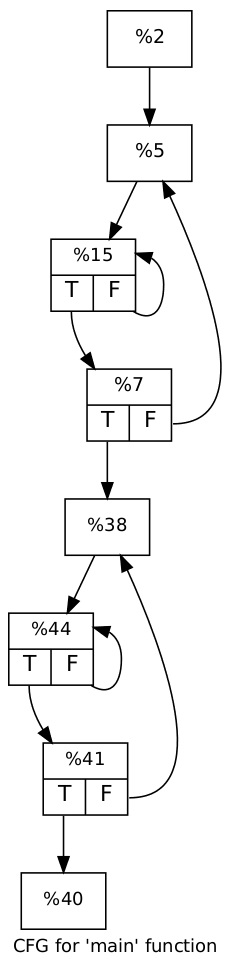
\includegraphics[width=\textwidth]{gfx/matmulCfg.png}
\end{figure}
Therefore the \cfg is very important to the pipeline as it is needed by many analysis passes and by optimization passes to determine whether certain optimizations can be applied and which way.
The current \cfg of a \llvmir file can be generated at any point of the pipeline.
It also can be visualized (like \autoref{fig:exampleCfg}) by passing one of the options \texttt{-view-cfg} or \texttt{-view-cfg-only} to the \opt.
\begin{enumerate}
    \item Translate the C++ sourcecode of \autoref{lst:matmulcpp} into \llvmir (\autoref{lst:matmulll})\\
        \texttt{clang++ -S -emit-llvm matmul.cpp -o matmul.ll}
    \item Generate the \cfg\\
        \texttt{opt -view-cfg matmul.ll}
\end{enumerate}

\chapter{Polly}
Polly\footnote{Der Name Polly ist eine Kombination von \enquote{Polyhedral} und \enquote{\ac{LLVM}} \cite{PollyGrosser}} ist eines der zahlreichen Unterprojekte der \ac{LLVM} und stellt Möglichkeiten bereit, automatische Optimierungen auf Basis des Polyedermodells auf \ac{LLVM-IR} durchzuführen.
Diese Optimierungen können über Flags des \ac{LLVM} Optimizers genutzt werden.
\section{Geschichte}
Polly wurde mit der Veröffentlichung (\cite{PollyGrosser}) eingeführt. TODO Mehr Informationen?

\section{Pipeline \cite{PollyPresentation}}
Die Einbindung von Polly wird über den \ac{LLVM} Optimizer realisiert, indem die Bibliothek von Polly geladen wird (\autoref{subsec:optimizer}).
\begin{figure}[h]
    \caption{Die Pipeline von Polly}
    \centering
    \begin{tikzpicture}
        \coordinate(clang);
        \node(opt)[llvmIrNode, right=of clang]{\ac{LLVM} Optimizer};
        \node(polly)[llvmIrNode, below=of opt]{\ac{LLVM} Polly};
        \coordinate[right=of opt](generator);
        \path[llvmIrPath] (clang) to (opt);
        \path[llvmIrPath, bend right] (opt.south west) to node[auto, swap]{SCoP Detection} (polly);
        \path[llvmIrPath, bend right] (polly) to node[auto, swap]{Code Generation} (opt.south east);
        \path[llvmIrPath] (opt) to (generator);
        \path[llvmIrPath] (polly) edge[loop below] ();
    \end{tikzpicture}
\end{figure}\\
Zwei essentielle Begriffe von Polly sind \enquote{Region} und \enquote{\ac{SCoP}}.
\subsection{Definition Region}

\subsection{Definition SCoP}


\cleardoublepage
%\ctparttext{\draftnote{Some additional text describing the study}}
\part{Empirical Study}
\chapter{Experiment Setup And Execution}
\section{Goals}

\section{Measurement Methology}
\draftnote{What is measured?
    \begin{itemize}
        \item ratio sequential and parallel instructions
        \item reasons for parents of SCoPs being invalid as SCoP
        \item Theoretical impact if certain reasons would not appear
    \end{itemize}
}
\subsection{Definition ratios}
Let \(S_s\in\mathbb{N}\) be the number of instructions not within a \scop, \(P_s\in\mathbb{N}\) the number of instructions within a \scop and \(I\in\mathbb{N}\) the number of all instructions such that \(S_s + P_s = I\).
Then the ratio of non-\scops is defined as:
\[RS_{seq} := \frac{S_s}{I}\]
And the \scop ratio is defined as:
\[RS_{par} := \frac{P_s}{I}\]
Let \(S_p\in\mathbb{N}\) be the number of instructions not within a parent of a \scop, \(P_p\in\mathbb{N}\) the number of instructions within a parent of a \scop and \(I\in\mathbb{N}\) the number of all instructions such that \(S_p + P_p = I\).
Then the not-parent-of-\scop ratio is defined as:
\[RP_{seq} := \frac{S_p}{I}\]
Analogue the parent-of-\scop ratio is defined as:
\[RP_{par} := \frac{P_p}{I}\]
\subsection[Amdahl's Law]{Amdahl's Law \cite{AmdahlsLaw}}
Let \(N\in\mathbb{N}\) be the number of processors and \(R_{seq}\in\mathbb{Q}\) be the sequential ratio.
Then the speedup \(S\in\mathbb{Q}\) is defined as:
\[S := \frac{N}{(R_{seq}*N)+(1-R_{seq})}\]
\subsection{Reasons for SCoPs being invalid}
These are the implemented criteria of Polly for rejecting a parent of a \scop being also a \scop.
\begin{itemize}
    \item Parent is toplevel (\autoref{lst:parentIsToplevel})
    \item Unsupported terminator instruction
    \item Unreachable in exit block (\autoref{lst:unreachableExitBlock})
    \item Irreducible loops (\autoref{lst:irreducibleLoops})
    \item Undefinded branch condition
    \item Non-integer branch condition
    \item Undefined operands in comparison
    \item Non-affine branch condition
    \item No base pointer
    \item Undefinded base pointer
    \item Variant base pointer (\autoref{lst:variantBasePointer})
    \item Non-affine memory accesses (\autoref{lst:nonAffineMemoryAccesses})
    \item Accesses with differing sizes
    \item Uncomputable loop bounds (\autoref{lst:uncomputeableLoopBounds})
    \item Loop without exit (\autoref{lst:loopWithoutExit})
    \item Function call with side effects (\autoref{lst:functionCallSideEffects})
    \item Complicated access semantics (volatile or atomic)
    \item Base address aliasing (\autoref{lst:baseAddressAliasing})
    \item Integer to pointer conversion (\autoref{lst:integerToPointer})
    \item Stack allocations
    \item Unknown instructions
    \item Contains entry block
    \item Assumed to be unprofitable (\autoref{lst:assumedUnprofitable})
\end{itemize}

\begin{comment}
    Following is copy\&pasted from pollys ScopDetectionDiagnostic.cpp

SCOP_STAT(CFG, ""),
SCOP_STAT(InvalidTerminator, "Unsupported terminator instruction"),
SCOP_STAT(UnreachableInExit, "Unreachable in exit block"),
SCOP_STAT(IrreducibleRegion, "Irreducible loops"),
SCOP_STAT(LastCFG, ""),
SCOP_STAT(AffFunc, ""),
SCOP_STAT(UndefCond, "Undefined branch condition"),
SCOP_STAT(InvalidCond, "Non-integer branch condition"),
SCOP_STAT(UndefOperand, "Undefined operands in comparison"),
SCOP_STAT(NonAffBranch, "Non-affine branch condition"),
SCOP_STAT(NoBasePtr, "No base pointer"),
SCOP_STAT(UndefBasePtr, "Undefined base pointer"),
SCOP_STAT(VariantBasePtr, "Variant base pointer"),
SCOP_STAT(NonAffineAccess, "Non-affine memory accesses"),
SCOP_STAT(DifferentElementSize, "Accesses with differing sizes"),
SCOP_STAT(LastAffFunc, ""),
SCOP_STAT(LoopBound, "Uncomputable loop bounds"),
SCOP_STAT(LoopHasNoExit, "Loop without exit"),
SCOP_STAT(FuncCall, "Function call with side effects"),
SCOP_STAT(NonSimpleMemoryAccess,
          "Compilated access semantics (volatile or atomic)"),
SCOP_STAT(Alias, "Base address aliasing"),
SCOP_STAT(Other, ""),
SCOP_STAT(IntToPtr, "Integer to pointer conversions"),
SCOP_STAT(Alloca, "Stack allocations"),
SCOP_STAT(UnknownInst, "Unknown Instructions"),
SCOP_STAT(Entry, "Contains entry block"),
SCOP_STAT(Unprofitable, "Assumed to be unprofitable"),
SCOP_STAT(LastOther, "")
\end{comment}

\section{Experiment Variables}
\begin{table}[H]
    \myfloatalign
    \begin{tabularx}{\textwidth}{Xccccc} \toprule
        \tableheadline{Name} & \tableheadline{Abbr.} & \tableheadline{Type} & \tableheadline{Scale Type} & \tableheadline{Unit} & \tableheadline{Range} \\ \midrule
        Ratio non-\scop & \(RS_{seq}\) & ? & Ratio & \% & \([0, 100]\)\\
        Ratio \scop & \(RS_{par}\) & ? & Ratio & \% & \([0, 100]\)\\
        Ratio non-parent-of-\scop & \(RP_{seq}\) & ? & Ratio & \% & \([0, 100]\)\\
        Ratio parent-of-\scop & \(RP_{par}\) & ? & Ratio & \% & \([0, 100]\)\\
        Speedup & \(S\) & ? & Ratio & ? & \(\mathbb{Q}\)\\
        \bottomrule
    \end{tabularx}
    \caption{Experiment Variables}
\end{table}

\section{Hypotheses}

\section{Subject Programs}
\begin{table}[H]
    \myfloatalign
    \begin{tabularx}{\textwidth}{XcX} \toprule
        \tableheadline{Name} & \tableheadline{Version} & \tableheadline{Tested Inputs} \\ \midrule
        benchbuild\\
        llvm\\
        clang\\
        polly\\
        polli\\ \midrule
        7z\\
        Rasdam\\
        bzip2\\
        ccrypt & & Integrated tests\\
        crafty & & Integrated benchmark\\
        crocopat & & Integrated benchmark\\
        ffmpeg\\
        gzip\\
        js\\
        lammps & & Integrated sample problems\\
        lapack & & Integrated tests\\
        leveldb & & Integrated benchmark\\
        libressl\\
        linpack & & Integrated benchmark\\
        lulesh & & Integrated benchmark\\
        lulesh-omp & & Integrated benchmark\\
        mcrypt & & Integrated benchmark\\
        minisat\\
        openblas\\
        postgres & & Integrated benchmark\\
        povray & & Integrated sample scenes\\
        python\\
        ruby\\
        sqlite3 & & leveldb's integrated benchmark\\
        tcc\\
        x264 & & Integrated benchmark\\
        xz\\
        \bottomrule
    \end{tabularx}
    \caption[Subject programs]{Subject programs and benchbuild used. (Versions in parenthesis represent git hashes)}
\end{table}

\section{Tasks}
\draftnote{
    \begin{enumerate}
        \item Create Pass (\autoref{subsec:optimizer})
        \begin{itemize}
            \item How does the pass work?
        \end{itemize}
        \item Run benchbuild over the group \enquote{benchbuild}
        \item Analyse output
            \begin{itemize}
                \item Most common reasons for rejection?
                \item Ratio of SCoPs?
                \item Possible effect when theoretically solve reasons for rejection?
            \end{itemize}
    \end{enumerate}
}

\section{Design}

\section{Experiment Setting}

\section{Deviations}

\section{Analyse}

%\addtocontents{toc}{\protect\clearpage} % <--- just debug stuff, ignore
%\include{multiToC} % <--- just debug stuff, ignore for your documents

\cleardoublepage
\part{Evaluation}
\chapter{Analysis}
\section{Descriptive Statistics}
\subsection{Ratios and Speedups}
The measurements taken are listed in \autoref{tab:ratiosAndSpeedups}.
\begin{table}[!ht]
    \resizebox{!}{\textwidth}{
        \begin{minipage}{\textwidth}
            \myfloatalign
            \begin{tabularx}{\textwidth}{Xcccc} \toprule
        \tableheadline{Project} & \tableheadline{\(R_s\)} & \tableheadline{\(R_p\)} & \tableheadline{\(S_s\)} & \tableheadline{\(S_p\)}\\\midrule
                \midrule
                \textbf{Benchmarks}\\
                MultiSourceApplications & - & - & - & -\\
                MultiSourceBenchmarks & - & - & - & -\\
                SingleSourceBenchmarks & - & - & - & -\\
                SPEC2006 & - & - & - & -\\
                Povray & - & - & - & -\\
                \midrule
                \textbf{Compression}\\
                7z & - & - & - & -\\
                bzip2 & - & - & - & -\\
                gzip & - & - & - & -\\
                xz & - & - & - & -\\
                \midrule
                \textbf{Database}\\
                Leveldb & - & - & - & -\\
                PostgreSQL & - & - & - & -\\
                SQLite3 & - & - & - & -\\
                \midrule
                \textbf{Encryption}\\
                ccrypt & - & - & - & -\\
                libressl & - & - & - & -\\
                \midrule
                \textbf{Multimedia}\\
                ffmpeg & - & - & - & -\\
                povRAY & - & - & - & -\\
                x264 & - & - & - & -\\
                \midrule
                \textbf{Scientific}\\
                LAMMPS & - & - & - & -\\
                LAPACK & - & - & - & -\\
                LINPACK & - & - & - & -\\
                \midrule
                \textbf{Simulation}\\
                crafty & - & - & - & -\\
                lulesh & - & - & - & -\\
                lulesh-omp & - & - & - & -\\

                \midrule
                \textbf{Verification}\\
                minisat & - & - & - & -\\
                \midrule
                \textbf{Other}\\
                js & - & - & - & -\\
                openblas & - & - & - & -\\
                Rasdaman & - & - & - & -\\
                \bottomrule
            \end{tabularx}
            \caption{Measured ratios and speedups}
            \label{tab:ratiosAndSpeedups}
        \end{minipage}
    }
\end{table}
\subsection{Reasons for rejecting parents}
The chart on \autoref{fig:rejectReasonsGrouped} visualizes the reasons for parents being reject as valid \scops.
\piechart{
      46.6/Chrome,
      24.6/Internet Explorer,
      20.4/Firefox,
      5.1/Safari,
      1.3/Opera,
      2.0/Other
}{Reasons for parents being rejected}{fig:rejectReasonsGrouped}
\section{Hypothesis Testing}

% ********************************************************************
% Backmatter
%*******************************************************
\appendix
%\renewcommand{\thechapter}{\alph{chapter}}
\cleardoublepage
\part{Appendix}
%********************************************************************
% Appendix
%*******************************************************
% If problems with the headers: get headings in appendix etc. right
%\markboth{\spacedlowsmallcaps{Appendix}}{\spacedlowsmallcaps{Appendix}}
\chapter{Appendix}
This chapter contains mainly lots of the source code and complete tables of data referenced within the study.
The main purpose is for getting an even more detailed impression of the used or generated files and for being able accurate reproducing the results of the study.
%\graffito{More dummy text.}

\section{Code Listings}
\subsection{Matmul.cpp Code Listings}
The following listings contain the (generated) code of the example matrix multiplication which is often used throuout the background chapters.
\begin{code}
    \caption{LLVM-IR of \autoref{lst:matmulcpp}}
    \inputminted{LLVM}{ll/matmul.ll}
    \label{lst:matmulll}
\end{code}
\begin{code}
    \caption{LLVM-IR (O3 optimized) of \autoref{lst:matmulcpp}}
    \inputminted{LLVM}{ll/matmulO3.ll}
    \label{lst:matmulllO3}
\end{code}
\begin{code}
    \caption{LLVM-IR of \autoref{lst:matmulcpp} prepared for Polly}
    \inputminted{LLVM}{ll/matmul.preopt.ll}
    \label{lst:matmulpreoptll}
\end{code}
\begin{code}
    \caption[Program for checking overhead]{The program used for checking the overhead of the measurement itself}
    \inputminted{c++}{cpp/checkMeasurementOverhead.cpp}
    \label{lst:checkOverhead}
\end{code}

\subsection{Examples for invalid SCoPs}
These peaces of code illustrate simple situations where \scops are invalid.
\begin{code}
    \caption{Parent is toplevel}
    \inputminted{c++}{cpp/ParentIsTopLevelRegion.cpp}
    \label{lst:parentIsToplevel}
\end{code}
\begin{code}
    \caption{Unreachable in exit block}
    \inputminted{c++}{cpp/UnreachableInExitBlock.cpp}
    \label{lst:unreachableExitBlock}
\end{code}
\begin{code}
    \caption{Irreducible loops}
    \inputminted{c++}{cpp/IrreducibleRegion.cpp}
    \label{lst:irreducibleLoops}
\end{code}
\begin{code}
    \caption{Variant base pointer}
    \inputminted{c++}{cpp/VariantBasePointer.cpp}
    \label{lst:variantBasePointer}
\end{code}
\begin{code}
    \caption{Non-affine memory accesses}
    \inputminted{c++}{cpp/NonAffineMemoryAccesses.cpp}
    \label{lst:nonAffineMemoryAccesses}
\end{code}
\begin{code}
    \caption{Uncomputable loop bounds}
    \inputminted{c++}{cpp/UncomputableLoopBounds.cpp}
    \label{lst:uncomputeableLoopBounds}
\end{code}
\begin{code}
    \caption{Loop without exit}
    \inputminted{c++}{cpp/LoopWithoutExit.cpp}
    \label{lst:loopWithoutExit}
\end{code}
\begin{code}
    \caption{Function call with side effects}
    \inputminted{c++}{cpp/FunctionCall.cpp}
    \label{lst:functionCallSideEffects}
\end{code}
\begin{code}
    \caption{Base address aliasing}
    \inputminted{c++}{cpp/BaseAddressAliasing.cpp}
    \label{lst:baseAddressAliasing}
\end{code}
\begin{code}
    \caption{Integer to pointer conversion}
    \inputminted{c++}{cpp/IntegerToPointerConversion.cpp}
    \label{lst:integerToPointer}
\end{code}
\begin{code}
    \caption{Assumed to be unprofitable}
    \inputminted{c++}{cpp/AssumedToBeUnprofitable.cpp}
    \label{lst:assumedUnprofitable}
\end{code}

\section{Specifications of machine used for measurements}
\begin{code}
    \captionsetup{type=table}
    \inputminted{text}{gfx/zeusLscpu.log}
    \caption[Specifications of the CPUs used for measurement]{
        Specifications of the CPUs used for measurement.
        More precisely it is simply the output of \texttt{lscpu}.
    }
    \label{tab:lscpu}
\end{code}
\begin{code}
    \captionsetup{type=table}
    \inputminted{text}{gfx/zeusMeminfo.log}
    \caption[Specifications of the memory of the machine used for measurement]{
        Specifications of the memory of the machine used for measurement.
        More precisely this is the output of \texttt{cat /proc/meminfo}.
    }
    \label{tab:meminfo}
\end{code}

\section{Data Tables}\label{sec:dataTables}
Here is the hole data listed collected throuout the entire study.
\LTXtable{\textwidth}{tables/ratiosScops.tex}
\LTXtable{\textwidth}{tables/ratiosMaxRegions.tex}
\LTXtable{\textwidth}{tables/invalidReasons.tex}

\begin{comment}
    \section{Appendix Section Test}
    Test: \autoref{tab:moreexample} (This reference should have a
    lowercase, small caps \spacedlowsmallcaps{A} if the option
    \texttt{floatperchapter} is activated, just as in the table itself
     $\rightarrow$ however, this does not work at the moment.)

    \begin{table}[h]
        \myfloatalign
      \begin{tabularx}{\textwidth}{Xll} \toprule
        \tableheadline{labitur bonorum pri no} & \tableheadline{que vista}
        & \tableheadline{human} \\ \midrule
        fastidii ea ius & germano &  demonstratea \\
        suscipit instructior & titulo & personas \\
        %postulant quo & westeuropee & sanctificatec \\
        \midrule
        quaestio philosophia & facto & demonstrated \\
        %autem vulputate ex & parola & romanic \\
        %usu mucius iisque & studio & sanctificatef \\
        \bottomrule
      \end{tabularx}
      \caption[Autem usu id]{Autem usu id.}
      \label{tab:moreexample}
    \end{table}

    \section{Another Appendix Section Test}
    Equidem detraxit cu nam, vix eu delenit periculis. Eos ut vero
    constituto, no vidit propriae complectitur sea. Diceret nonummy in
    has, no qui eligendi recteque consetetur. Mel eu dictas suscipiantur,
    et sed placerat oporteat. At ipsum electram mei, ad aeque atomorum
    mea. There is also a useless Pascal listing below: \autoref{lst:useless}.

    \begin{lstlisting}[float=b,language=Pascal,frame=tb,caption={A floating example (\texttt{listings} manual)},label=lst:useless]
    for i:=maxint downto 0 do
    begin
    { do nothing }
    end;
    \end{lstlisting}
\end{comment}

%********************************************************************
% Other Stuff in the Back
%*******************************************************
\cleardoublepage\nocite{*}

%********************************************************************
% Bibliography
%*******************************************************
% work-around to have small caps also here in the headline
\manualmark
\markboth{\spacedlowsmallcaps{\bibname}}{\spacedlowsmallcaps{\bibname}} % work-around to have small caps also
%\phantomsection
\refstepcounter{dummy}
\addtocontents{toc}{\protect\vspace{\beforebibskip}} % to have the bib a bit from the rest in the toc
\addcontentsline{toc}{chapter}{\tocEntry{\bibname}}
\label{app:bibliography}
\begin{sloppypar}
    \printbibliography
\end{sloppypar}

\cleardoublepage%*******************************************************
% Declaration
%*******************************************************
\refstepcounter{dummy}
\pdfbookmark[0]{Declaration}{declaration}
\chapter*{Declaration}
\thispagestyle{empty}
\draftnote{
I declare that I have developed and written the enclosed Bachelor Thesis completely by myself, and have not used sources or means without declaration in the text.
Any thoughts from others or literal quotations are clearly marked.
The Bachelor Thesis was not used in the same or in a similar version to achieve an academic grading or is being published elsewhere.\\
http://www.wiwiss.uni-jena.de/wiwimedia/Dokumente/Fakultaet/Zentrale\_Einrichtungen/Pruefungsamt/Statutory+Declaration.pdf
}
\bigskip
 
\noindent\textit{\myLocation, \myTime}

\smallskip

\begin{flushright}
    \begin{tabular}{m{5cm}}
        \\ \hline
        \centering\myName \\
    \end{tabular}
\end{flushright}

\cleardoublepage\pagestyle{empty}

\hfill

\vfill


\pdfbookmark[0]{Colophon}{colophon}
\section*{Colophon}
This document was typeset using the typographical look-and-feel \texttt{classicthesis} developed by Andr\'e Miede. 
The style was inspired by Robert Bringhurst's seminal book on typography ``\emph{The Elements of Typographic Style}''. 
\texttt{classicthesis} is available for both \LaTeX\ and \mLyX: 
\begin{center}
\url{https://bitbucket.org/amiede/classicthesis/}
\end{center}
Happy users of \texttt{classicthesis} usually send a real postcard to the author, a collection of postcards received so far is featured here: 
\begin{center}
\url{http://postcards.miede.de/}
\end{center}
 
\bigskip

\noindent\finalVersionString

%Hermann Zapf's \emph{Palatino} and \emph{Euler} type faces (Type~1 PostScript fonts \emph{URW
%Palladio L} and \emph{FPL}) are used. The ``typewriter'' text is typeset in \emph{Bera Mono}, 
%originally developed by Bitstream, Inc. as ``Bitstream Vera''. (Type~1 PostScript fonts were made 
%available by Malte Rosenau and
%Ulrich Dirr.)

%\paragraph{note:} The custom size of the textblock was calculated
%using the directions given by Mr. Bringhurst (pages 26--29 and
%175/176). 10~pt Palatino needs  133.21~pt for the string
%``abcdefghijklmnopqrstuvwxyz''. This yields a good line length between
%24--26~pc (288--312~pt). Using a ``\emph{double square textblock}''
%with a 1:2 ratio this results in a textblock of 312:624~pt (which
%includes the headline in this design). A good alternative would be the
%``\emph{golden section textblock}'' with a ratio of 1:1.62, here
%312:505.44~pt. For comparison, \texttt{DIV9} of the \texttt{typearea}
%package results in a line length of 389~pt (32.4~pc), which is by far
%too long. However, this information will only be of interest for
%hardcore pseudo-typographers like me.%
%
%To make your own calculations, use the following commands and look up
%the corresponding lengths in the book:
%\begin{verbatim}
%    \settowidth{\abcd}{abcdefghijklmnopqrstuvwxyz}
%    \the\abcd\ % prints the value of the length
%\end{verbatim}
%Please see the file \texttt{classicthesis.sty} for some precalculated 
%values for Palatino and Minion.
%
%    \settowidth{\abcd}{abcdefghijklmnopqrstuvwxyz}
%    \the\abcd\ % prints the value of the length





% ********************************************************************
% Game Over: Restore, Restart, or Quit?
%*******************************************************
\end{document}
% ********************************************************************
